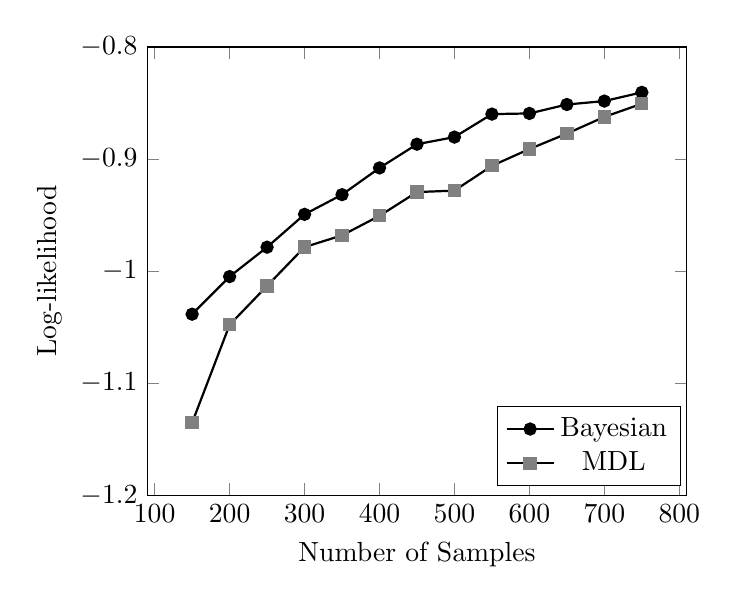
\begin{tikzpicture}
\begin{axis}[
		xlabel = Number of Samples,
		ylabel = Log-likelihood,
		legend style={at={(0.99,0.02)},anchor=south east},
		ymin= -1.2, ymax= -0.8
]
\addplot+[solid ,black,thick, mark options={black}] coordinates {
(150,	-1.03842)
(200,	-1.00487)
(250,	-0.978629)
(300,	-0.949342)
(350,	-0.931778)
(400,	-0.907931)
(450,	-0.886758)
(500,	-0.880402)
(550,	-0.859904)
(600,	-0.859312)
(650,	-0.851338)
(700,	-0.848281)
(750,	-0.840507)
};
\addlegendentry{Bayesian};

\addplot+[solid ,black,thick, mark options={black!50}] coordinates {
(150,	-1.13526)
(200,	-1.04789)
(250,	-1.01318)
(300,	-0.978555)
(350,	-0.968083)
(400,	-0.950671)
(450,	-0.92945)
(500,	-0.928194)
(550,	-0.906013)
(600,	-0.891075)
(650,	-0.877307)
(700,	-0.862388)
(750,	-0.850656)
};
\addlegendentry{MDL};
\end{axis}
\end{tikzpicture}
